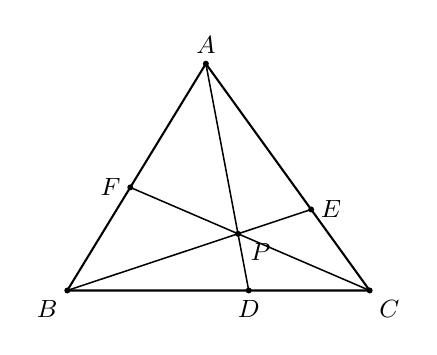
\begin{tikzpicture}[scale=0.80, line cap=round, line join=round, every node/.style={font=\small}]
    \coordinate (A) at (0,3.6);
    \coordinate (B) at (-2.2,0);
    \coordinate (C) at (2.6,0);
    \coordinate (D) at ({17/25},0);
    \coordinate (E) at ({117/70},{9/7});
    \coordinate (F) at ({-6/5},{18/11});
    \coordinate (P) at (0.51,0.9);
    \draw[line width=0.75pt] (A)--(B)--(C)--cycle;
    \draw[line width=0.55pt] (A)--(D) (B)--(E) (C)--(F);
    \foreach \X in {A,B,C,D,E,F,P} {\fill (\X) circle (1.35pt);}
    \node[above] at (A) {$A$};
    \node[below left] at (B) {$B$};
    \node[below right] at (C) {$C$};
    \node[below] at (D) {$D$};
    \node[right] at (E) {$E$};
    \node[left] at (F) {$F$};
    \node[below right,xshift=1pt] at (P) {$P$};
\end{tikzpicture}
